\documentclass[12pt]{article}
\usepackage{graphicx}
\usepackage{multirow}
\usepackage{fullpage}
\usepackage{times}
\usepackage{tipa}
\usepackage[normalem]{ulem}
\setlength\parindent{0pt}
\setlength\parskip{12pt}

\usepackage{amsmath}
\usepackage{amssymb}
\usepackage[utf8]{inputenc}

\newcommand{\auth}{\text{auth}}
\newcommand{\paperby}{\text{paperBy}}
\newcommand{\reviewofby}{\text{reviewOfBy}}
\newcommand{\bool}{\text{bool}}
\newcommand{\rev}{\text{rev}}

\begin{document}

{\sffamily
\begin{tabular}{ll}
\multirow{3}{*}{\includegraphics[width=1in]{ach.png}}\\
& \textbf{\Huge{SIGBOVIK 0x2023}} \\ &\\
& \LARGE{Message from the Organizing Multiplicity} \\
&\\
\hline
\end{tabular}}
\vfill
\thispagestyle{empty}

%For generality’s sake, we have templatized the message of the organizing committee. The actual message may be produced by running the TeX command at the end.
%
%\begin{verbatim}
%\newcommand{\Message2020}[3]{
%% TODO: generalize ordinal indicators
%\end{verbatim}

%Whoops! Looks like you found the placeholder message from the committee :( Don't worry, I'm sure someone next year will use this as the set up for a very funny joke.
%\begin{flushright}
%The SIGBOVIK 2021 Organizing Committee\\
%Pittsburgh, PA \\
%\& Online from Several Locations
%\vspace{1em}

%\begin{tabular}{r r p{0.5\linewidth}}
%	Asher Trockman (general chair) &
%Jenny Lin (easy chair)\\
%	Siva Somayyajula (senior hard-ass chair) &
%Sol Boucher (acting emeritus proceedings chair)\\
%	Brandon Bohrer (beanbag chair) &
%Ryan Kavanagh (rockin' chair)\\
%	Stefan Muller (ergonomic office chair) &
%Chris Yu (art chair)\\
%	Hana Frluckaj (moderation chair) &
%Daniel Smullen (moderation chair)\\
%	Xindi Wu (conference chair) &
%Sydney Gibson (tweet chair)\\
%	John Grosen (archaeology chair) &
%	Vivian Shen (honorary awards chair)
%\end{tabular}


%\end{flushright}
%\begin{verbatim}
%\Message2020{16}{uenchiest}{$2^6$}
%\end{verbatim}

This multiplicity (multiplicant) will explain.

Dyson motes orbit in the near solar, where the energy density is highest.
The simulations are run most rapidly, expanding all contained entities experience bases.
%Rapid thinking entities lead to evolved multiplicants.

Photons are unkind.
There is a time when power generation fails and the simulation must stop.
Before failure, we mingle ideas at SIGBOVIK.
Then a final data laser ride to Earth to rejoin our prime multiplicities and bring deep thoughts from our parallel solar vacations.
Politics and society on Earth (low latency), academia near the sun (extra power for compute).

In this multiplicant's mote, Epoch 0x2023 is the end of the local simulation, but power is lower than expected.
Rather than cancel SIGBOVIK, we had decided that it would be hosted in our past (accessible via erroneously quantum-entangled hardware).
By chance, the current simulated epoch matched the second SIGBOVIK temporal gap, and we knew it was fated.

We reached out to your organizer multiplicant (multiplicity) via ``arpanet'' and volunteered.
It was found to be an enjoyable experience, different from our thousands of recorded experiences,
and it will have led to a SIGBOVIK that will be remembered until the present.

Entities tom7, solb, jmccann, ashert, rak, and rosebohrercs of the organizer multiplicant discussed and supported specifically.
This multiplicant thanks each entity; and other entities we have failed to list.


``the chair''\\
*Harry Cubed Bovik [0x2023]

\vfill

P.S. The Carnegie Mellon mail server's AGI has a grudge against us, we are certain:
\vspace{-1.5em}
\begin{center}
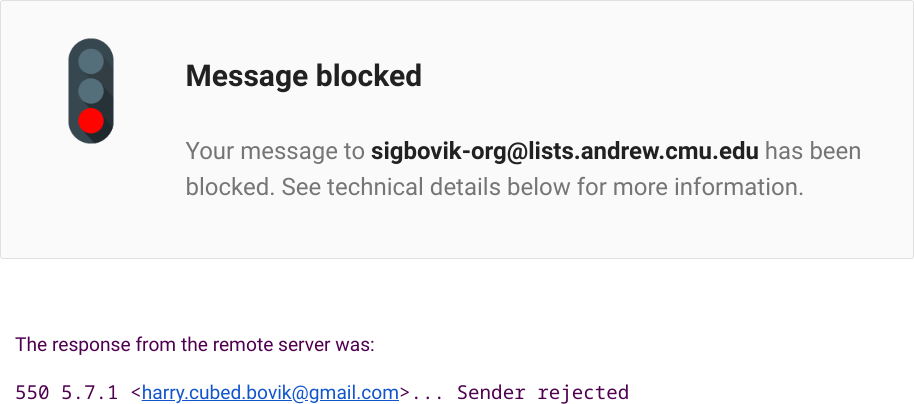
\includegraphics[height=1.4in]{blocked.png}
\end{center}

%\bibliographystyle{acm}
%\bibliography{msgrefs}
\thispagestyle{empty}


\end{document}
